\subsection{平方根形状的有界自然梯度与显式动力学}

由式~\eqref{eq:proximal-natural-velocity}，$\|v_\kappa\|_F^2=\Var_q(\rho^\kappa)/\kappa^2$。当 $0<\kappa\le1/2$，$2\kappa\le1$，Jensen 不等式给出 $\E_q\rho^{2\kappa}\le(\E_q\rho)^{2\kappa}=1$，于是
\begin{equation}
 \|v_\kappa\|_F^2\le\frac{1-A_\kappa^2}{\kappa^2}\le\frac1{\kappa^2}.
 \label{eq:proximal-natural-speed-bound}
\end{equation}
该界对任意完整支持的 $q,t$ 成立，不需要给 teacher 或 student 指定统一概率下界。对于 $\kappa>1/2$，取 $q=(\varepsilon,1-\varepsilon)$、$t=(c,1-c)$，$0<c<1$ 固定，则
\begin{equation}
 \Var_q(\rho^\kappa)
 =\varepsilon(1-\varepsilon)
 \left[(c/\varepsilon)^\kappa-((1-c)/(1-\varepsilon))^\kappa\right]^2
 \sim c^{2\kappa}\varepsilon^{1-2\kappa}\longrightarrow\infty.
\end{equation}
几何端点 $\kappa=0$ 也没有统一界：固定 $q=(1/4,3/4)$、令 $t=(\varepsilon,1-\varepsilon)$，$\Var_q\log(t/q)$ 随 $\varepsilon\to0$ 发散。故 $0<\kappa\le1/2$ 是这个自然梯度族具有统一 Fisher 速度界的区间。确定性的 Fisher 速度与随机参数梯度方差是不同对象，不能把这个结论直接写成完整训练梯度的方差定理。

在平方根点 $\kappa=1/2$，$A=\sum\sqrt{qt}$，并有 $\E_q\rho=1$，因此
\begin{equation}
 \|v_{1/2}\|_F^2=4(1-A^2)\le4,\qquad
 D_{1/2}(t\Vert q)=4(1-A).
\end{equation}
由 Lyapunov 等式，连续流满足
\begin{equation}
 \frac{dA}{d\tau}=1-A^2,
 \qquad A(\tau)=\tanh(\tau+\operatorname{artanh}A(0)),\quad q\ne t.
 \label{eq:proximal-hellinger-flow}
\end{equation}
证明是 $dD_{1/2}/d\tau=-4\,dA/d\tau=-4(1-A^2)$，然后积分 $dA/(1-A^2)=d\tau$。$q=t$ 时 $A=1$ 且流恒定。进一步，$D'=-(1+A)D$，由于 $0<A\le1$，有
\begin{equation}
 D(0)e^{-2\tau}\le D(\tau)\le D(0)e^{-\tau}.
\end{equation}
若写 $A=\cos\vartheta$，则 $d\vartheta/d\tau=-\sin\vartheta$。平方根形状既有球面解释，也有显式 teacher 接近度和有界 Fisher 速度。这使它成为一个有数学依据的候选点，尚不能据此断言其训练性能优于其他形状。

\begin{figure}[htbp]
 \centering
 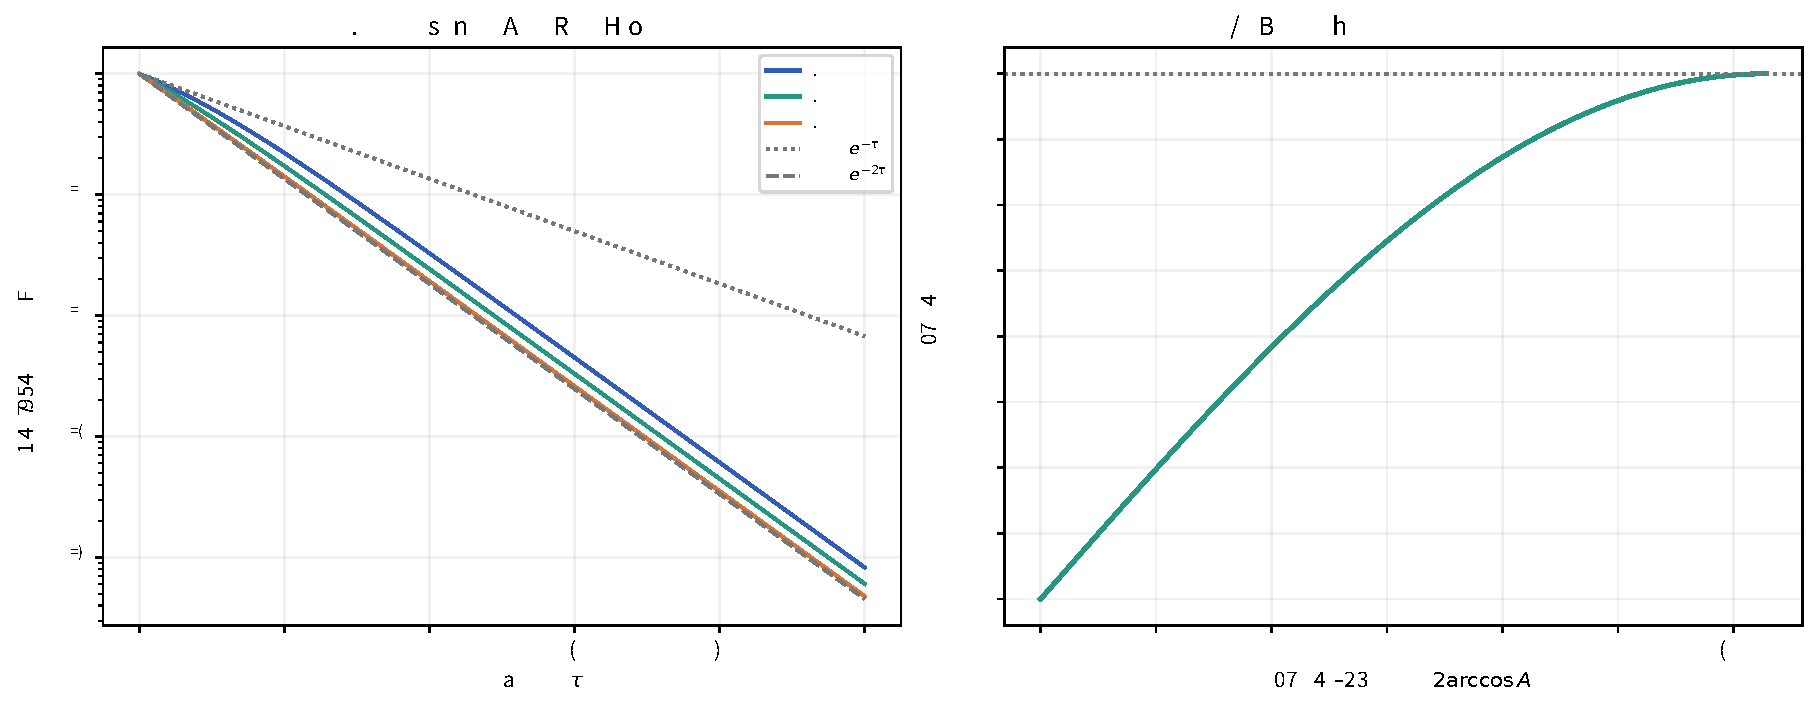
\includegraphics[width=\textwidth]{../../results/proximal-family-geometry/hellinger-flow.pdf}
 \caption{平方根形状的连续动力学。左图由 $A(\tau)=\tanh(\tau+\operatorname{artanh}A(0))$ 精确生成，归一化散度位于两个指数包络之间；右图将 Fisher 速度写成到 teacher 的 Fisher--Rao 距离函数，展示统一上界 2。}
\end{figure}

\subsection{小插值强度的最坏二阶矩存在形状阈值}

固定 $\kappa>0$ 时，上节使用的统一 $O(\lambda)$ 界还可以加强。这里考察完整支持概率分布上的最坏即时信号二阶矩
\begin{equation}
 \mathcal B_\kappa(\lambda)
 =\sup_{q,t}\E_q\left[
 \left(\frac1\kappa\log(1-\lambda+\lambda(t/q)^\kappa)\right)^2
 \right].
\end{equation}
上界对任何有限维数成立；下界的二元见证已足够。它是未标准化的冻结信号，不含 student 残差。

\begin{theorem}[最坏二阶矩的精确小强度阶数]
\label{thm:proximal-moment-threshold}
对任意固定 $0<\kappa\le1$，当 $\lambda\to0$ 时
\begin{equation}
 \mathcal B_\kappa(\lambda)=\Theta_\kappa\left(\lambda^{\min\{2,1/\kappa\}}\right).
 \label{eq:proximal-sharp-moment-order}
\end{equation}
$\Theta_\kappa$ 中的常数可依赖 $\kappa$，不依赖词表维数。几何端点则满足 $\mathcal B_0(\lambda)=\infty$，对任意 $\lambda>0$ 成立。
\end{theorem}

\begin{proof}
记 $\rho=t/q$。负区域 $\rho<1$ 的二阶矩不超过 $\log^2(1-\lambda)/\kappa^2=O_\kappa(\lambda^2)$。在正区域，$0\le f\le\log(1+\lambda\rho^\kappa)/\kappa$。

若 $0<\kappa\le1/2$，用 $\log(1+x)\le x$ 与 $\E_q\rho^{2\kappa}\le1$ 得到
\begin{equation}
 \E_q[f^2\mathbf1\{\rho\ge1\}]
 \le\frac{\lambda^2}{\kappa^2}\E_q\rho^{2\kappa}
 \le\frac{\lambda^2}{\kappa^2}.
\end{equation}
所以 $\mathcal B_\kappa(\lambda)\le[\log^2(1-\lambda)+\lambda^2]/\kappa^2=O_\kappa(\lambda^2)$。取任一固定完整支持且 $q\ne t$ 的二元分布，逐项 Taylor 展开给出 $f/\lambda\to(\rho^\kappa-1)/\kappa$。有限项求和后 $\E_qf^2/\lambda^2\to\E_q(\rho^\kappa-1)^2/\kappa^2>0$，得到匹配的下界。

若 $1/2<\kappa\le1$，令 $s=1/\kappa\in[1,2)$。常数 $C_s=\sup_{x>0}\log^2(1+x)/x^s$ 有限，因为比值在零点按 $x^{2-s}$ 趋零，在无穷处也趋零。于是
\begin{equation}
 \E_q[f^2\mathbf1\{\rho\ge1\}]
 \le\frac{C_s\lambda^s}{\kappa^2}\E_q\rho^{\kappa s}
 =\frac{C_s\lambda^{1/\kappa}}{\kappa^2}.
\end{equation}
负区域的 $O(\lambda^2)$ 比这个阶数更小。为证明下界，取 $t=(1/2,1/2)$、$q_1=\tfrac12\lambda^{1/\kappa}$、$q_2=1-q_1$。第一项满足 $\rho_1=\lambda^{-1/\kappa}$、$f_1=\log(2-\lambda)/\kappa$，所以
\begin{equation}
 \E_qf^2\ge q_1f_1^2
 =\frac{\lambda^{1/\kappa}}{2\kappa^2}\log^2(2-\lambda)
 =\Omega_\kappa(\lambda^{1/\kappa}).
\end{equation}
上下界匹配。$\kappa=1/2$ 已由第一种情况覆盖，也可取 $s=2$、$C_2=1$。$\kappa=0$ 时 $f=\lambda\log(t/q)$，固定有正质量的 $q$ 并令对应 teacher 概率趋零，二阶矩无界。\hfill$\square$
\end{proof}

这个阶数区分了“固定分布的小步展开”与“对所有分布统一的小步上界”。固定 $q,t$ 时，对每个 $\kappa$ 都有 $\E_qf^2=O(\lambda^2)$；最坏情形允许 $q,t$ 随 $\lambda$ 改变，$\kappa>1/2$ 的稀有正尾部因此留下更慢的 $\lambda^{1/\kappa}$ 阶数。TOP-D 算术端点为 $\Theta(\lambda)$，平方根点为 $\Theta(\lambda^2)$，二者的差异来自采样二阶矩，不是两种学习率单位。

若 score 范数不超过 $M$，定理立即给即时 score 估计与精确条件中心化估计相同阶数的方差上界，因为 $\Var(\psi f)\le M^2\E_qf^2$、$\Var(\psi C_qf)\le M^2\E_qf^2$。它没有证明所有参数化模型都达到这个最坏阶数，也没有覆盖随机标准化后的信号。

\begin{figure}[htbp]
 \centering
 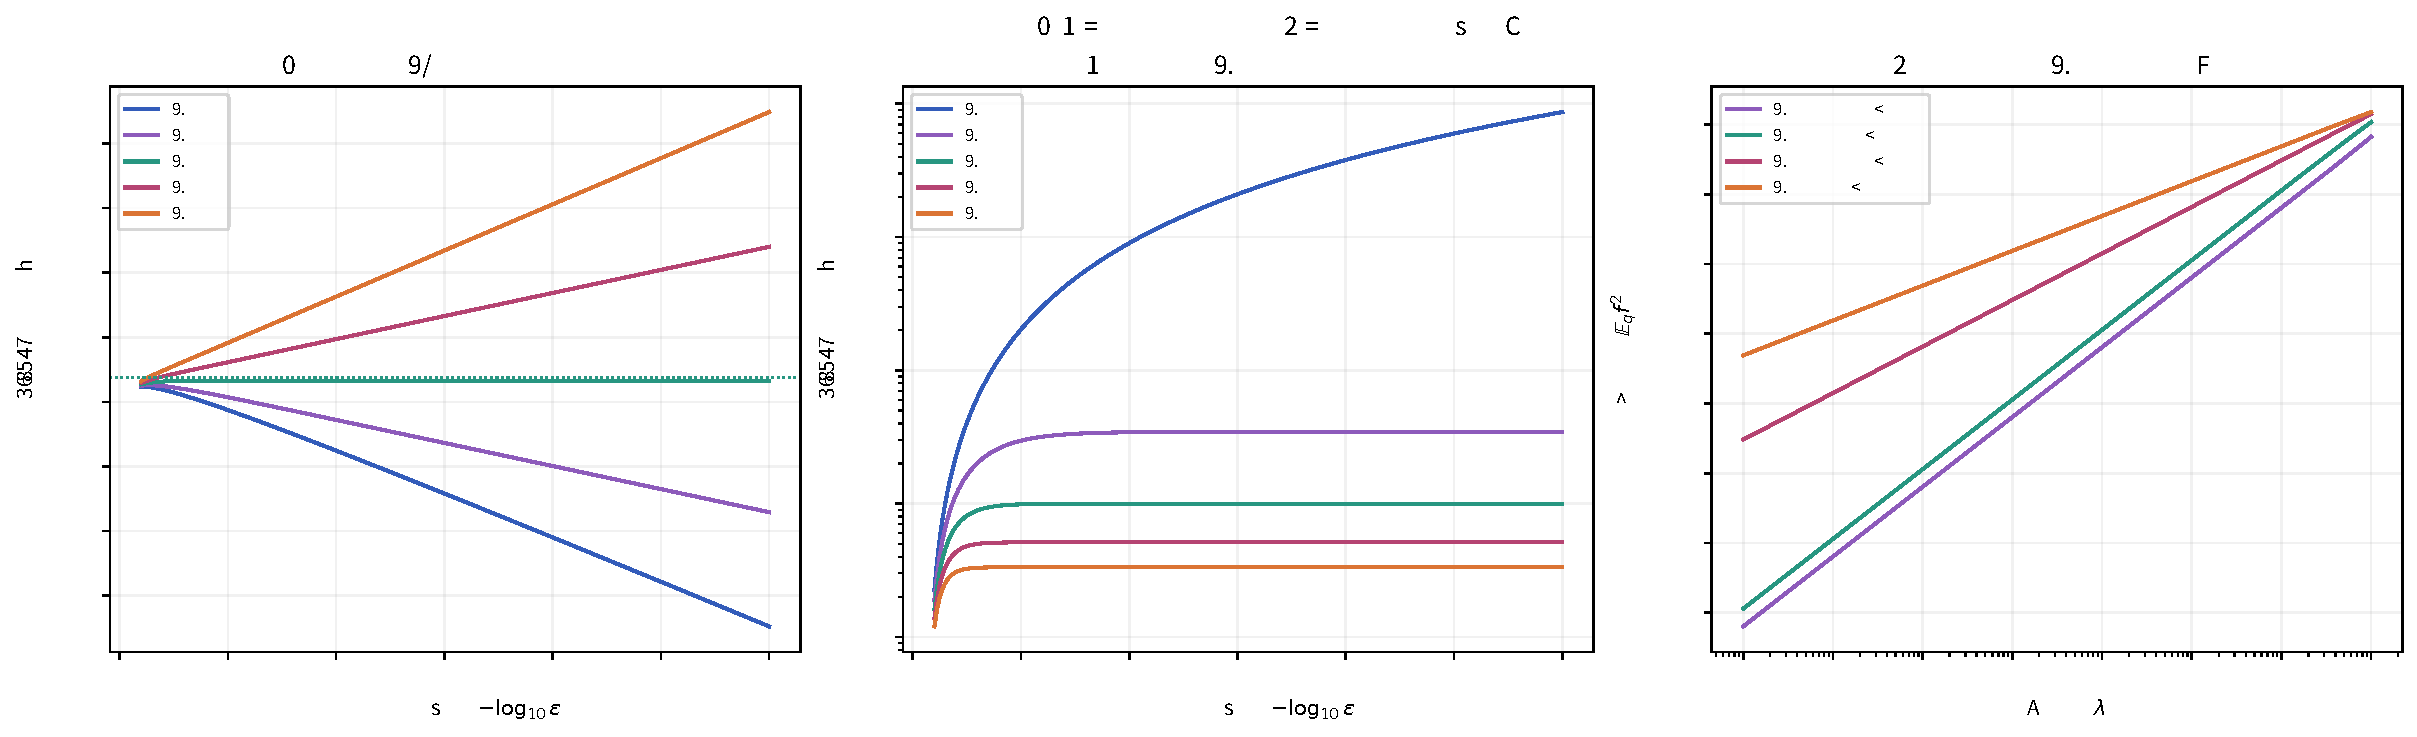
\includegraphics[width=\textwidth]{../../results/proximal-family-geometry/threshold.pdf}
 \caption{形状阈值的解析见证。左图让学生概率趋零，$\kappa>1/2$ 的自然梯度 Fisher 速度发散；中图让 teacher 概率趋零，几何端点的速度发散；右图使用随 $\lambda$ 改变的二元 anchor，信号二阶矩斜率分别趋于 $2,2,4/3,1$。右图不是对所有分布做数值最大化，其作用是验证证明中的下界见证。}
\end{figure}

\subsection{共享参数子流形上的自然梯度投影}

独立 token 分布的速度界还可延伸到共享参数的自然梯度流，但需要明确度量。取有限个 prefix、固定权重 $d_s>0$、$\sum_sd_s=1$，将外层分布写成 $q_\theta(a\mid s)>0$。定义
\begin{equation}
 L_\kappa(\theta)=\sum_sd_sD_\kappa(t_s\Vert q_{\theta,s}),\qquad
 \langle v,w\rangle_W=\sum_{s,a}\frac{d_s}{q_{\theta,s,a}}v_{s,a}w_{s,a}.
\end{equation}
记 $J=\partial q_\theta/\partial\theta$，$W=\operatorname{diag}(d_s/q_{\theta,s,a})$，则参数 Fisher 矩阵为 $\mathcal I=J^\top WJ$。令 $v$ 为每个 prefix 上的无约束负自然梯度，$v_{s,a}=q_{\theta,s,a}(\rho_{s,a}^\kappa-\E_{q_{\theta,s}}\rho_s^\kappa)/\kappa$。因为每个 prefix 的 $J$ 列向量分量和为零，$\nabla_\theta L=-J^\top Wv$。

参数自然梯度流采用 Moore--Penrose 广义逆 $\mathcal I^+$ 时，有
\begin{equation}
 \dot\theta=-\mathcal I^+\nabla_\theta L,\qquad
 \dot q_\theta=J\mathcal I^+J^\top Wv=Pv.
\end{equation}
$P$ 是到 $\operatorname{range}(J)$ 的 $W$ 正交投影：令 $B=W^{1/2}J$，则 $W^{1/2}PW^{-1/2}=B(B^\top B)^+B^\top$，后者是普通欧氏正交投影。因此
\begin{equation}
 \|\dot q_\theta\|_W^2\le\|v\|_W^2,\qquad
 \frac{dL}{d\tau}=-\langle v,Pv\rangle_W=-\|Pv\|_W^2\le0.
\end{equation}
平方根形状满足 $\|v\|_W^2=\sum_sd_s\,4(1-A_s^2)\le4$，所以共享参数的精确自然梯度流也满足 $\|\dot q_\theta\|_W\le2$。更一般地，$0<\kappa\le1/2$ 时平方速度不超过 $1/\kappa^2$。

这个结论控制的是分布流在固定 prefix Fisher 度量下的速度。它不控制参数的欧氏范数，也不自动适用于普通梯度流。共享参数还可能使 $Pv=0$ 而 $q_\theta\ne t$，因此单调性和速度界并不保证无投影误差的 teacher 收敛。离散幂均值 target 的精确 escort 轨迹也不会因这个局部投影结论自动延续到共享参数模型。

\subsection{平方根候选与尚待回答的数学问题}

三个独立结果支持优先研究 $\kappa=1/2$：它是 Hellinger 重心并沿 Fisher--Rao 短弧；连续流有显式 $A(\tau)$ 和 $\|v\|_F\le2$；小 $\lambda$ 的统一即时信号二阶矩为 $O(\lambda^2)$。$0<\kappa<1/2$ 也具有有界速度和相同最坏阶数，但上界常数、目标路径与 teacher 散度不同。$\kappa=1/2$ 是仍具有这两个统一矩性质的最大形状参数，尚不是在任何固定任务损失下证明的最优形状。

在 $0<\kappa\le1/2$ 内，所给速度平方上界 $1/\kappa^2$ 与信号二阶矩上界 $[\log^2(1-\lambda)+\lambda^2]/\kappa^2$ 都随 $\kappa$ 增大而减小，负信号下界 $\log(1-\lambda)/\kappa$ 则增大。平方根点在这一组统一界上有最小的上界和最温和的负下界。界的优劣不等于每个固定分布上的实际方差优劣，不能把这段比较替代固定评价目标下的最优性证明。

下一步的纯数学工作应区分目标选择与模型投影。固定一个外部评价散度后，研究不同 $\kappa$ 的有限步改进、曲率与噪声常数，才有可比较的优化问题；直接最小化各自不同的 $D_\kappa$ 数值不能给出通用最优 $\kappa$。共享参数策略族下，还需证明有限 inner 的拟合损失怎样控制 $D_\kappa(m\Vert p)$ 或 escort 误差，才能把精确外层结论应用到模型更新；上一小节的自然梯度投影只提供连续时间单调性和速度界。prefix 测度刷新是另一项独立条件。

新增图和精确求和核验由 \path{experiments/analysis/proximal_family_dynamics.py} 生成，数据和版本见 \path{results/proximal-family-geometry/dynamics-summary.json}。3、64、1024 维各五组随机概率向量检验超额损失分解、teacher 进展恒等式、escort 步和自然梯度流；有限差分另检验最优点的 Hessian 与 escort 流导数。共享参数核验使用三个 prefix、每个五个 action、四个共享参数的条件指数族，验证参数梯度、Fisher 正交投影和速度界。幂均值、原始散度和新的核验结论均保留完整支持条件。
